\documentclass[border=10pt]{standalone}
\usepackage{tikz}\usepackage{amsmath}\usetikzlibrary{arrows.meta}
\begin{document}
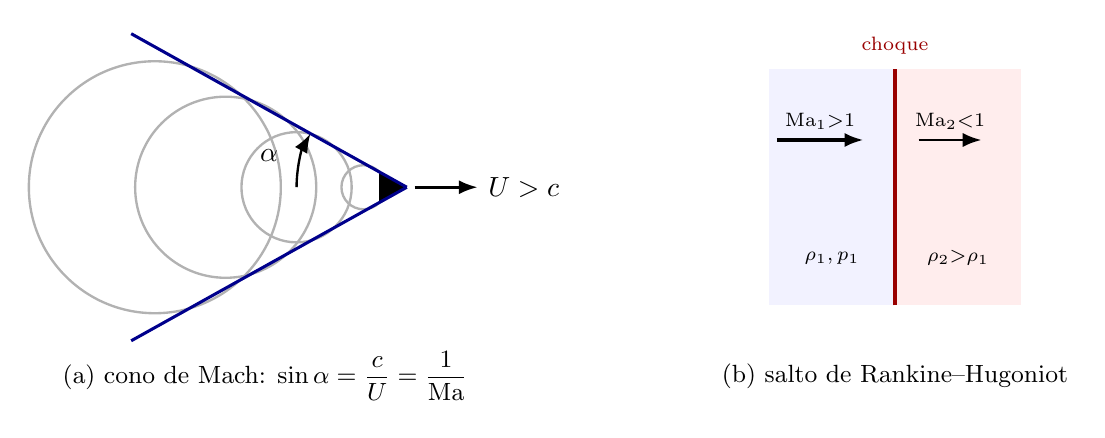
\begin{tikzpicture}[line width=0.85pt,>={Latex[length=2.4mm]}]
  % (a) cono de Mach
  \foreach \r/\x in {1.6/-3.2,1.15/-2.3,0.7/-1.4,0.28/-0.55}
     \draw[gray!60] (\x,0) circle(\r);
  \fill (0,0)--(-0.35,0.18)--(-0.35,-0.18)--cycle;
  \draw[->,line width=1pt] (0.1,0)--(0.9,0) node[right]{$U>c$};
  \draw[blue!55!black,line width=1.1pt] (0,0)--(-3.5,1.95); \draw[blue!55!black,line width=1.1pt] (0,0)--(-3.5,-1.95);
  \draw[->] (-1.4,0) arc (180:151:1.4); \node at (-1.75,0.4){$\alpha$};
  \node at (-1.8,-2.4){\small (a) cono de Mach: $\sin\alpha=\dfrac{c}{U}=\dfrac{1}{\mathrm{Ma}}$};
  % (b) onda de choque normal
  \begin{scope}[xshift=6.2cm]
    \fill[blue!5] (-1.6,-1.5) rectangle (0,1.5); \fill[red!7] (0,-1.5) rectangle (1.6,1.5);
    \draw[line width=1.3pt,red!60!black] (0,-1.5)--(0,1.5); \node[red!60!black] at (0,1.8){\scriptsize choque};
    \draw[->,line width=1.2pt] (-1.5,0.6)--(-0.4,0.6) node[midway,above]{\scriptsize$\mathrm{Ma}_1{>}1$};
    \draw[->,line width=1pt] (0.3,0.6)--(1.1,0.6) node[midway,above]{\scriptsize$\mathrm{Ma}_2{<}1$};
    \node at (-0.8,-0.9){\scriptsize$\rho_1,p_1$}; \node at (0.8,-0.9){\scriptsize$\rho_2{>}\rho_1$};
    \node at (0,-2.4){\small (b) salto de Rankine--Hugoniot};
  \end{scope}
\end{tikzpicture}
\end{document}
